Music, one of the oldest forms of art and entertainment humanity has ever had,
has played a significant role in different cultures and civilizations worldwide
since the beginning of history.

With the progress of artificial intelligence in many areas such as computer vision,
speech recognition, and natural language processing,
machine learning enthusiasts have tried
to use all their knowledge in music-related fields. \cite{musicCompositionML}

Artists tried different approaches to music composition,
from free playing and improvisation to diving deep into the
rhythm, notes, scales, modes, and other elements of music theory,
for both of them existing various approaches in machine learning.
This chapter explores several of these methods related to this paper's work,
but before immersing in the machine learning aspects, we should discuss how they process data.



\section{What is MIDI?}
MIDI (\textbf{M}usical \textbf{I}nstrument \textbf{D}igital \textbf{I}nterface) specifies a standard for connecting,
playing, and recording electronic instruments and a file format to store this information.
It uses messages in an event-driven manner,
meaning that each note is represented as an event that specifies its
notation, pitch, velocity, and other useful characteristics. \cite{midiCourse}

The MIDI file format is a popular choice among data scientist
when working with audio and music due to several aspects:

\begin{itemize}
    \item{
          \emph{ease of manipulation}:
          one can edit the parameters of a note without the need for rerecording; \cite{midiAmanda}
          }
    \item{
          \emph{ability to change instruments}:
          a MIDI file only defines what notes should be played and in which order,
          not the instrument that should perform them; \cite{midiAmanda}
          }
    \item{
          \emph{small size}: this file format is comparable to an electronic sheet;
          it does not hold any audio information,
          only instructions for playing the notes,
          saving a whole song in just several kilobytes of data. \cite{midiAmanda}
          }
\end{itemize}

\section{LakhNES and Transformer-XL}

One of the latest music-generation approaches is Chris Donahue's
\emph{LakhNES: Improving multi-instrumental music generation with cross-domain pre-training}.
The author uses language models and their ability to retain long-term sequences within the data,
being able to generate multi-instrumental structured songs. \cite{donahue2019lakhnes}


Before discussing his approach,
one must understand the insights of the used models.
Transformer-XL is a neural network used for resolving natural language processing tasks,
achieving state-of-the-art results on different language datasets.
Other proposals for these problems are models based on recurrent neural networks and long
short-term memory, which give great results on more straightforward data,
but cannot establish longer dependencies between words due to their limitations. \cite{transformerXLMedium}

\begin{figure}[h]
    \centering
    \includegraphics[width=1\textwidth]{Transformer_XL}
    \caption{\emph{Transformer-XL - training and evaluation \cite{transformerXLMedium}}}
    \label{fig:transformerXLMedium}
\end{figure}

Vanilla Transformers tend to resolve this problem by introducing new attention modules.
They receive a sequence of tokens (instead of processing tokens one by one)
and determine the connections between them based on absolute positional encoding.
The main obstacle with this network is that it can only receive
one sequence of specified length at a time;
hence, the data can suffer from context fragmentation. \cite{transformerXLMedium}


\begin{wrapfigure}{L}{0.5\textwidth}
    \centering
    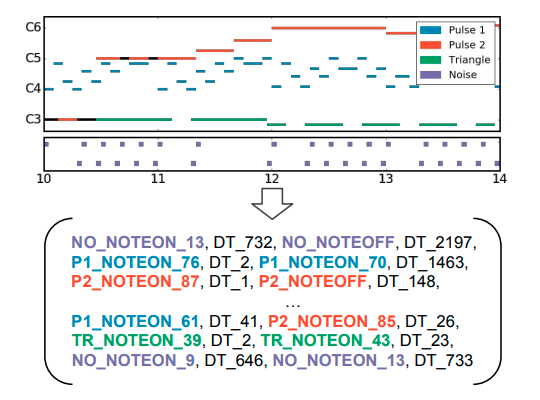
\includegraphics[width=0.45\textwidth]{lakhnessConversion}
    \caption{\emph{Note conversion example used in \cite{donahue2019lakhnes}}}
    \label{fig:noteConversion}
\end{wrapfigure}

Transformers-XL solves the problems mentioned above by
using relative positional encoding and a recurrence mechanism
to extend their context for much better and faster performance.
Figure\emph{~\ref{fig:transformerXLMedium}} represents a small outline of the training and evaluation phase of the discussed network,
in which one can observe how the extended context is created and used.




In \cite{donahue2019lakhnes}, they used the Transformer-XL,
by creating a grammar through which they converted the MIDI events
into text that the network can process.
An example of this conversion is in Figure\emph{~\ref{fig:transformerXLMedium}}.
In this manner,
they can convert any MIDI to some text with
which they train the model and then use it
for generating new complex structured songs or
completing existing ones.


Another noticeable aspect of their work is that they used
transfer learning, their purpose being to generate NES music game,
but, by using this approach of pre-training their model with
general standard data, they increased the performance of the model
by 10\%. \cite{donahue2019lakhnes}


\section{Composer and Autoencoders}
The main inspiration for this work is HackerPoet's \emph{Composer} \cite{hackerPoet},
another point of view for music generation that uses deep autoencoders.

As explained in the previous chapters,
this type of neural network learns in an unsupervised manner the internal representation of our data.
Using only the decoding part,
the author generates new MIDIs by feeding it new normalized encodings and predicting new songs.
He trained his model with game music utilizing a dataset that he created, his main goal being game themes. \cite{hackerPoet}

This approach has excellent results regarding music theory,
the model being able to compose songs with a well-defined structure,
having popular chord progressions, bassline, multiple melodies, and also musical motifs. \cite{hackerPoet}

The good results and the ease of understanding and implementing autoencoders are
the main reason they have been used in this application, one key difference in this paper's
approach being represented by the structure of our autoencoder and how the encoding was
enhanced with the emotional value from the dataset.


\section{AIVA - Artificial Intelligence Virtual Artist}

Another proposal worth mention is the algorithm behind the startup \emph{AIVA} \cite{aiva}.
It is a deep learning model that uses reinforcement learning,
initially and mainly trained on classical pieces based on compositions of great musicians
like Mozart, Beethoven, and Bach.
In the latest releases, it was also trained on different styles of music. \cite{aiva1}

It is the first artificial intelligence recognized as a composer by a copyright authority -
SACEM (standing for Society of Authors, Composers and Publishers of Music).
Therefore, its pieces are not public, their songs being copyrighted. \cite{aiva2}

AIVA's algorithm most essential features are creating new compositions or
finishing existing ones based on a given genre, or even writing with influences of another song.
In other words, it can learn the style of a piece and compose a song
in the same fashion as the input one.\cite{aiva1}
